\chapter{Overview}

% ToDo: 全体構成の模式図を入れる
\begin{figure}[htbp]
 \begin{center}
  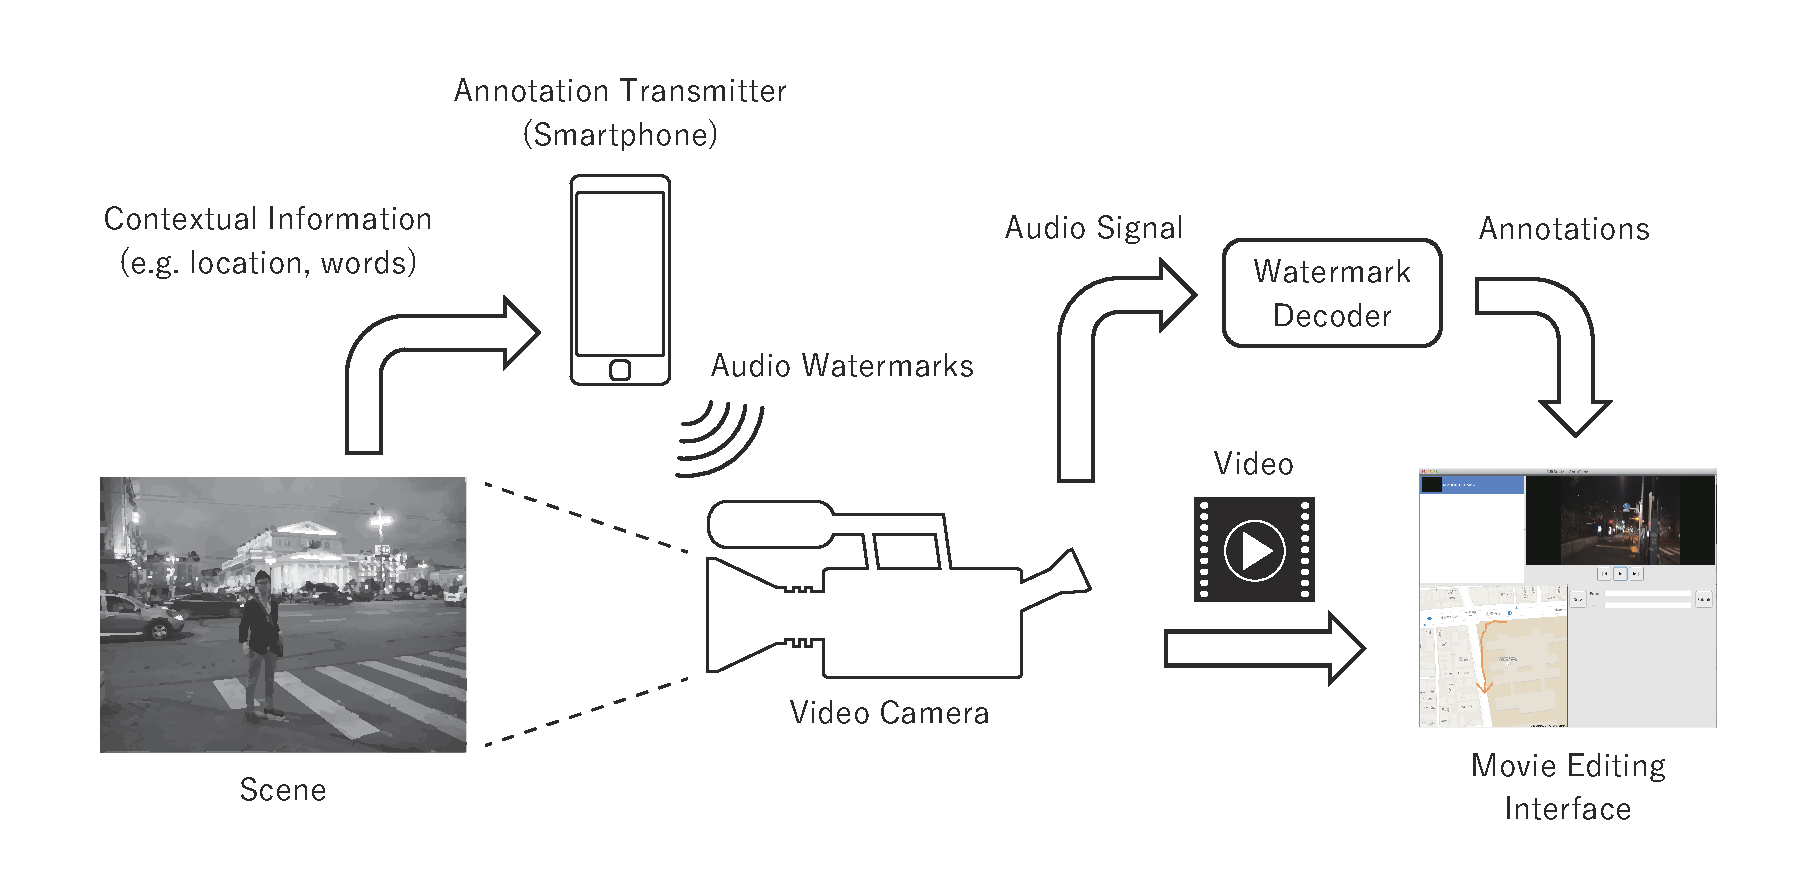
\includegraphics[width=150mm]{overview.pdf}
 \end{center}
 \caption{The schematic diagram of the system of AnnoTone}
 \label{fig:one}
\end{figure}

% AnnoToneのシステムは
% 1. アノテーションを生成するプログラム
% 2. アノテーションからWatermarkを生成するプログラムコンポーネント
% 3. Watermarkデコードを行うプログラムコンポーネント
% 4. アノテーションをもとに動画編集機能やUIを提供するプログラム
% によって構成される
The system of AnnoTone consists of four kinds of software components, those are watermark generator, watermark decoder, annotation interface and movie editing interface.
To guarantee the extensibility, we designed the system so that two interfaces can be implemented easily to realize new use of annotations using shared components for dealing with watermarks.

\section{Annotation Transmitter}
% 1と2でアノテーションレコーダーアプリを構成する
An annotation interface enables users to decide what to embed into a video as annotations, and sends them to a watermark generator to generate watermark signals representing them.
These two components comprise a smartphone application that transmits watermark signals from a back speaker of a smartphone to a microphone of a video camera.
The feature of the interface varies depending on the purpose of annotation.
It automatically makes annotations without any user operation if the purpose is to record a series of measured data like geolocation, otherwise it offers an user interface for users to explicitly embed annotations.

\section{Movie Editing Application}
% 3と4でビデオエディティングアプリを構成する
A watermark decoder and a movie editing interface constitute a software application that exploits embedded annotations for video editing.
The former take a video file imported from a video camera as an input and extracts annotations embedded into it as watermarks.
Extracted annotations are loaded into the movie editing interface, and offer its user a variety of functions for creating movie contents.
